\documentclass[a4paper,10pt]{book}
\usepackage[pdftex]{graphicx}
\usepackage{epstopdf}
\usepackage{subfigure}
\usepackage{amsmath,amsthm}
\usepackage{tikz}
\usepackage{circuitikz}
\usetikzlibrary{babel}
\usetikzlibrary{shapes, arrows, patterns, angles, quotes}
\textwidth= 15cm
\evensidemargin=0cm
\usepackage[spanish]{babel}
\usepackage[utf8]{inputenc}
\usepackage{textcomp}
\usepackage{amstext}
\usepackage{amsfonts}
\usepackage{amssymb}
\usepackage{comment}
\usepackage[hyperindex=true,breaklinks=true,colorlinks=true,linkcolor=blue]{hyperref}
\renewcommand{\tablename}{Tabla}
\renewcommand{\listtablename}{\'Indice de Tablas}
\usepackage{color}
\definecolor{gray97}{gray}{.97}
\definecolor{gray75}{gray}{.75}
\definecolor{gray45}{gray}{.45}
\usepackage{color} %red, green, blue, yellow, cyan, magenta, black, white
\definecolor{mygreen}{RGB}{28,172,0} % color values Red, Green, Blue
\definecolor{mylilas}{RGB}{170,55,241}

\usepackage{listings}
\lstloadlanguages{C,XML}
\lstset{ frame=Ltb,
	framerule=0pt,
	aboveskip=0.5cm,
	framextopmargin=3pt,
	framexbottommargin=3pt,
	framexleftmargin=0.8cm,
	framesep=0pt,
	rulesep=.4pt,
	backgroundcolor=\color{gray97},
	rulesepcolor=\color{black},
	%
	stringstyle=\ttfamily,
	showstringspaces = false,
	basicstyle=\small\ttfamily,
	commentstyle=\color{gray45},
	keywordstyle=\bfseries,
	%
	numbers=left,
	numbersep=15pt,
	numberstyle=\tiny,
	numberfirstline = false,
	breaklines=true,
}

% minimizar fragmentado de listados
\lstnewenvironment{listing}[1][]
{\lstset{#1}\pagebreak[0]}{\pagebreak[0]}

\lstdefinestyle{consola}
{basicstyle=\scriptsize\bf\ttfamily,
	backgroundcolor=\color{gray75},
}

\lstdefinestyle{C}
{language=C,
}

\lstdefinestyle{XML}
{language=XML,
}


\usepackage{multirow}
\usepackage{makeidx}

%\usepackage{draftwatermark}
%\SetWatermarkText{Borrador,juan.jimenez@fis.ucm.es}
%\SetWatermarkScale{2}

% Atajos para el tikz
\tikzstyle{block} = [draw, rectangle, minimum width=6em]
\tikzstyle{sum} = [draw, fill=blue!20, circle, node distance=1cm]
\tikzstyle{input} = [coordinate]
\tikzstyle{output} = [coordinate]
\tikzstyle{pinstyle} = [pin edge={to-,thin,black}]

% Entornos para los "teoremas"
\newtheorem{algo}{Algoritmo}[section]
\newtheorem{theorem}{Teorema}[section]
\newtheorem{problem}{Problema}[section]
\newtheorem{corollary}{Corolario}[section]
\newtheorem{lemmas}{Lema}[section]
\newcommand*{\lema}{Lema}
\newenvironment{lemma}[1][\lema]{\begin{lemmas}[#1]\renewcommand*{\qedsymbol}{\(\Diamond\)}}{\end{lemmas}}

\theoremstyle{definition}
%\newtheorem{definition}{Definición}[section]
\newtheorem{definitions}{Definición}[section]
\newcommand*{\definicion}{Definición}
\newenvironment{definition}[1][\definicion]{\begin{definitions}[#1]\renewcommand*{\qedsymbol}{\(\bigtriangledown\)}}{\end{definitions}}

\newtheorem{examples}{Ejemplo}[section]
\newcommand*{\ejemplo}{Ejemplo}
\newenvironment{example}[1][\ejemplo]{\begin{examples}[#1]\renewcommand*{\qedsymbol}{\(\maltese\)}}{\end{examples}}
%\renewcommand{\qedsymbol}{\maltese}

\theoremstyle{remark}
\newtheorem{remark}{Atención}[section]

\graphicspath{{./figuras/}}
\makeindex
\begin{document}
\title{
\begin{flushleft}

\includegraphics[width=2.5cm]{ucm2.eps}
Universidad Complutense de Madrid\\
---------------------------------------------------------------------\
\end{flushleft}
Manual de Paparazzi}
\author{ UCM237}

\maketitle\
\
\vspace*{\fill}

\includegraphics[scale=1]{by-sa.eps}\\
El contenido de estos apuntes est\'e1 bajo licencia Creative Commons Atribution-ShareAlike 4.0\\
\href{http://creativecommons.org/licenses/by-sa/4.0/}{http://creativecommons.org/licenses/by-sa/4.0/}\\
\copyright Juan Jim\'enez

\bigskip
\tableofcontents
\listoffigures
%\listoftables
%\section*{Matlab Code}
\lstset{language=Matlab,%
    %basicstyle=\color{red},
    breaklines=true,%
    morekeywords={matlab2tikz},
    keywordstyle=\color{blue},%
    morekeywords=[2]{1}, keywordstyle=[2]{\color{black}},
    identifierstyle=\color{black},%
    stringstyle=\color{mylilas},
    commentstyle=\color{mygreen},%
    showstringspaces=false,%without this there will be a symbol in the places where there is a space
    numbers=left,%
    numberstyle={\tiny \color{black}},% size of the numbers
    numbersep=9pt, % this defines how far the numbers are from the text
    emph=[1]{for,end,break},emphstyle=[1]\color{red}, %some words to emphasise
    %emph=[2]{word1,word2}, emphstyle=[2]{style},    
}

Esto es un simple guía burros para paparazzi, dado que entender lo que dice es complicadillo.
En principio, podemos dividirlo en capítulos, y emplear para cada uno un archivo nuevo.

De todos modos, lo importante es ir escribiendo y luego vemos como organizarlo. \\

Antes de comenzar, indicar que a lo largo de todo este documento vamos a trabajar con Linux, más concretamente con el sistema operativo Ubuntu en su versión 20.04. Este es el único entorno que va a soportar PaparazziUAV.\\

\noindent El equipo que desarrolla PaparazziUAV cuenta con una wiki muy detallada que puede llegar a ser muy útil para incorporarse al entorno: \url{https://wiki.paparazziuav.org/wiki}. Para instalar PaparazziUAV recomendamos al usuario seguir directamente la entrada \textit{installation} (\url{https://wiki.paparazziuav.org/wiki/Installation}) y leer el \textit{README.md} principal del proyecto (\url{https://github.com/UCM-237/paparazzi}). \\
\chapter{Paparazzi Center}

% TODO: ¿Sección de instalación?

\noindent Una vez realizada la instalación, podremos ejecutar el binario precompilado \textit{paparazzi} que se encuentra en la carpeta raíz de Paparazzi. Entonces se inicializará todo el ecosistema y se ejecutará Paparazzi Center, el panel de control principal de PaparazziUAV [Figura \ref{fig:cap1_interfaz}]. En él nos encontraremos inicialmente con un proyecto (A/C) ejemplo. Dentro de cada proyecto podremos introducir varios \textbf{archivos de configuración .xml} (en el capítulo sobre el directorio \textit{conf} explicaremos más detalladamente para qué sirve cada uno):

\begin{enumerate}
    \item \textbf{Airframe}: va a contener toda la información sobre el hardware y firmware de nuestro vehículo. \url{https://wiki.paparazziuav.org/wiki/Airframe_Configuration}.
    
    \item \textbf{Flight Plan}: definirá la geolocalización, los bloques y los waypoints que aparecerán en el modo navegación.
    
    \item \textbf{Radio}: ajustará las ganancias y la funcionalidad de los canales del radio control. Paparazzi ya trae la configuración de varios modelos, si nuestro controlador no se encuentra entre ellos deberemos de generar su .xml teniendo en cuenta sus especificaciones.
    
    \item \textbf{Telemetry}: definirá los distintos modos de telemetría del vehículo y los mensajes que se enviarán en cada uno de ellos. 
    
\end{enumerate}

\begin{figure}[h!]
    \centering
    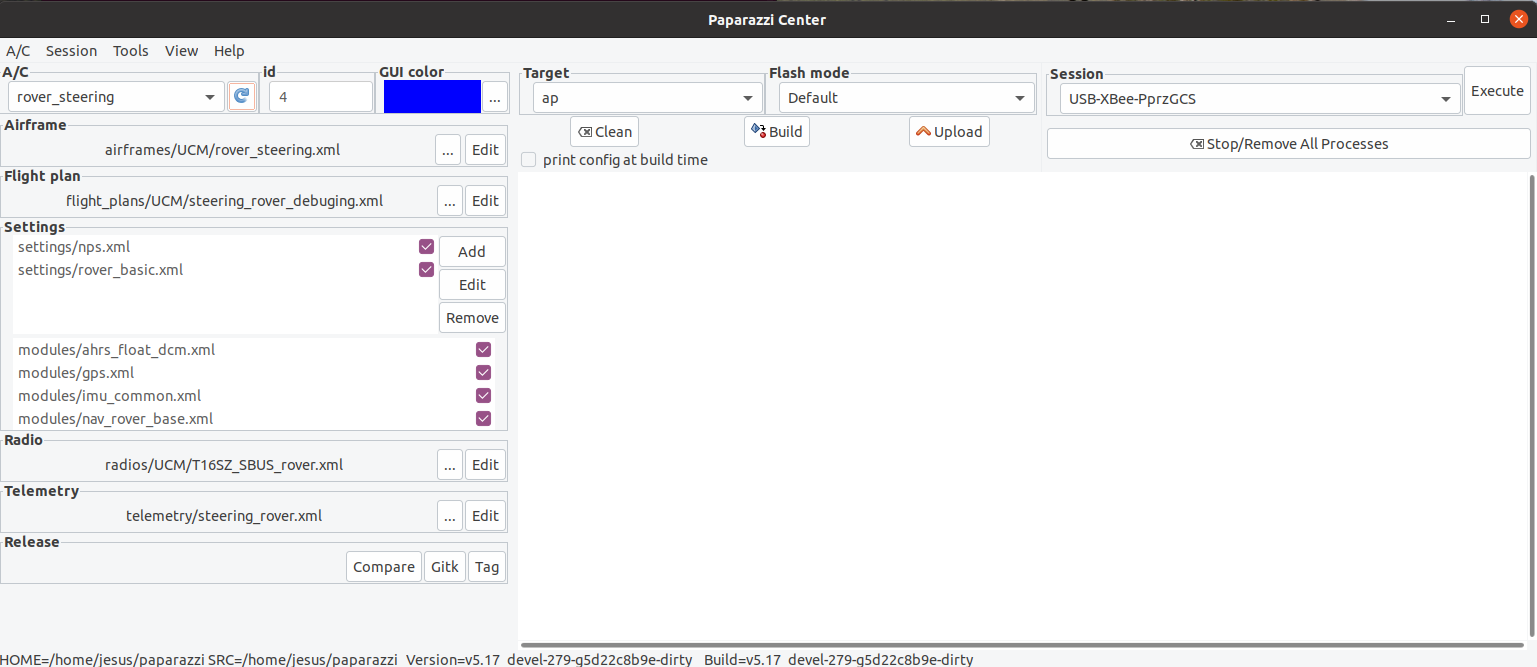
\includegraphics[width=0.8\textwidth]{./figuras/cap1_interfaz.png}
    \caption{Interfaz de Paparazzi Center, el panel de control principal de PaparazziUAV.} \label{fig:cap1_interfaz}
\end{figure}

\newpage

Para compilar ... \\

Herramientas y sesiones ... \\


\chapter{Ground control station} 
\chapter{El directorio conf}
\chapter{El directorio sw}
\chapter{Un ejemplo completo: Rover Steering}
\chapter{Módulo de comunicación serie}

El módulo de comunicación serie permite que Paparazzi establezca comunicación bidireccional con otro dispositivo a través de uno de los puertos serie. Con este módulo implementaremos el protocolo de comunicaciones entre paparazzi y la Raspberry (o el companion computer) correspondiente.

\section{Protocolo de comunicación}\label{sec:1}

La comunicación entre Paparazzi y el (companion Computer) CC será bidireccional. Todos los mensajes llevarán una marca de tiempo. Los mensajes establecidos son los siguientes:
\begin{enumerate}
	\item Mensajes desde Paparazzi al CC
	\begin{enumerate}
		\item Mensaje con los datos de telemetría. 
		\item Mensaje indicando al CC que puede proceder a realizar las medidas.
		\item Mensaje solicitando al CC la posición de la sonda.
	\end{enumerate}
	\item Mensajes desde el CC al Paparazzi
	\begin{enumerate}
			\item Mensaje de respuesta a la solicitud de medida.
			\item Mensaje periódico con la profundidad de la sonda (durante la medida).
			\item Mensaje de finalización de medida.
			\item Mensaje de respuesta a la solicitud de posición de la sonda con la posición.
	\end{enumerate}	
\end{enumerate}

\subsection{Configuración del puerto serie}

La configuración del puerto serie será la estándar con velocidad de $9600$ baudios, tabla \ref{tab:1}.
\begin{table}[h]
	\centering
	\caption{Configuración del puerto serie}
\begin{tabular}{|c|c|}
	\hline
	\textbf{Parámetro} & \textbf{Valor} \\ \hline \hline
	Velocidad  & $9600$ (baudios) \\\hline 
	Paridad & ninguna  \\ \hline
	Bits & $8$ \\ \hline 
	Bits de parada & $1$  \\ \hline
	Control de flujo & ninguno \\ \hline
\end{tabular}
\label{tab:1}
\end{table}


\subsection{Comunicación desde paparazzi}

Paparazzi enviará tres mensajes diferentes al CC. Uno de ellos periódico, el mensaje de la telemetría y el resto puntualmente.

Todos los mensajes comienzan con un byte que contiene el código ASCII de la letra \textbf{P} indicando que dicho mensaje procede de paparazzi. Todos los mensajes terminan con $2$ bytes que corresponden al checksum.

Las cantidades numéricas enteras sin signo se codifican usando el formato Little Endian (el byte más significativo ocupa la posición de menor índice en el mensaje). Por ejemplo si queremos enviar el número decimal $72$ como hexadecimal de $2$ bytes lo codificaremos como: $\{0x00,0x48\}$.

Las cantidades numéricas con signo se codifican de igual manera que las enteras sin signo pero el byte de menor índice se usa para indicar el signo: $0x01$ si el signo es negativo y $0x00$ si es positivo. Por ejemplo si usamos $3$ bytes para codificar el número $-72$ lo codificaremos como $\{0x01,0x00,0x48\}$ y el número $72$ será $\{0x00,0x00,0x48\}$.

\subsubsection{Mensaje de telemetría}

El mensaje de telemetría es un mensaje periódico que envía paparazzi al CC con los datos de telemetría: GPS y medida de Sonar. Tiene una longitud de $25$ bytes y la estructura en bytes especificada en la tabla \ref{tab:2}.

\begin{table}[h]
	\centering
	\caption{Estructura del mensaje de telemetría}
	\begin{tabular}{|c|c|c|c|}\hline 
		\textbf{Posición}	& \textbf{Valor} & \textbf{Tipo} &\textbf{Número de bytes} \\ \hline \hline 
		$0$		& Byte de sincronía ``P''				& ASCII	 			&	$1$ \\  \hline
		$1$		& Tipo de mensaje ``T''				& ASCII	 			&	$1$ \\  \hline
		$2-3$	& Marca de tiempo (s)				& Entero sin signo	&   $2$ \\  \hline
		$4-8$	& Longitud ($grad \cdot 10^{7}$)	& Entero con signo	&   $5$ \\  \hline
		$9-13$	& Latitud ($grad \cdot 10^{7}$)		& Entero con signo	&  	$5$ \\  \hline
		$14-17$	& Altitud ($mm$)					& Entero sin signo	&   $4$ \\  \hline
		$18-21$	& Distancia sonar ($mm$)			& Entero sin signo	&   $4$ \\  \hline
		$22$	& Confianza sonar ($\%$)			& Entero sin signo	&   $1$ \\  \hline
		$23-24$	& Checksum 							& Entero sin signo	&   $2$ \\  \hline
	\end{tabular}
	\label{tab:2}
\end{table}

En la tabla \ref{tab:3} puede verse un ejemplo de uno de estos mensajes.

\begin{table}
	\centering
	\caption{Ejemplo de un mensaje de telemetría}
	\begin{tabular}{|c|c|c|c|}\hline
		\textbf{Byte} 	&	\textbf{Valor (en hexadecimal)}	&\textbf{Valor}	&\textbf{Significado} \\ \hline \hline
		$0$ 			&  $0x50$			& ``P''	& Byte sincronía	\\ \hline
		$1$				&  $0x54$			& ``T''	& Tipo mensaje		\\ \hline
		$2$				&  $0x00$			& \multirow{2}{*}{$72$ segundos} & \multirow{2}{*}{Tiempo} \\
		$3$				&  $0x48$			&  & \\ \hline	
		$4$				&  $0x01$			&  \multirow{5}{*}{$-37260579$ ($grad \cdot 10^{7}$) } &  \multirow{5}{*}{Longitud}  \\
		$5$				&  $0x02$			&  &   \\ 	
		$6$				&  $0x38$			&  &    \\ 	
		$7$				&  $0x8D$			&  &    \\ 	
		$8$				&  $0x23$			&   &   \\ \hline
		$9$				&  $0x00$			& \multirow{5}{*}{$404506308$ ($grad \cdot 10^{7}$) } &  \multirow{5}{*}{Latitud}   \\
		$10$				&  $0x18$			&  &     \\ 	
		$11$				&  $0x1C$			&  &      \\ 	
		$12$				&  $0x46$			&  &      \\ 	
		$13$				&  $0xC4$			&  &      \\ \hline
		$14$				&  $0x00$			& \multirow{4}{*}{$702385$ (mm) } & \multirow{4}{*}{Altitud}\\
		$15$				&  $0x0A$			&   &     \\ 	
		$16$				&  $0xB7$			&   &         \\ 	
		$17$				&  $0xB1$			&   &        \\ \hline
		$18$				&  $0x00$			& \multirow{4}{*}{$8219$ (mm) } & \multirow{4}{*}{Distancia sonar}\\
		$19$				&  $0x00$			&     &     \\ 	
		$20$				&  $0x20$			&     &     \\ 	
		$21$				&  $0x1B$			&     &     \\ 	\hline
		$22$				&  $0x64$			& $100 \%$ &     Confianza \\ \hline
		$23$				&  $0x05$			&  \multirow{2}{*}{6405}	& \multirow{2}{*}{checksum} \\
		$24$				&  $0x19$			&     &     \\ \hline	
		
		
	\end{tabular}
	\label{tab:3}
\end{table}

\subsubsection{Mensaje indicando al CC que puede proceder a realizar las medidas}

El mensaje de inicio de medidas es un mensaje puntual que envía paparazzi al CC indicando que puede comenzar a descender la sona para tomar medidas. Incluye los datos de telemetría: GPS y medida de Sonar. Tiene una longitud de $25$ bytes y la estructura en bytes especificada en la tabla \ref{tab:4}.

\begin{table}[h]
	\centering
	\caption{Estructura del mensaje de inicio de medida}
	\begin{tabular}{|c|c|c|c|}\hline 
		\textbf{Posición}	& \textbf{Valor} & \textbf{Tipo} &\textbf{Número de bytes} \\ \hline \hline 
		$0$		& Byte de sincronía ``P''				& ASCII	 			&	$1$ \\  \hline
		$1$		& Tipo de mensaje ``M''				& ASCII	 			&	$1$ \\  \hline
		$2-3$	& Marca de tiempo (s)				& Entero sin signo	&   $2$ \\  \hline
		$4-8$	& Longitud ($grad \cdot 10^{7}$)	& Entero con signo	&   $5$ \\  \hline
		$9-13$	& Latitud ($grad \cdot 10^{7}$)		& Entero con signo	&  	$5$ \\  \hline
		$14-17$	& Altitud ($mm$)					& Entero sin signo	&   $4$ \\  \hline
		$18-21$	& Distancia sonar ($mm$)			& Entero sin signo	&   $4$ \\  \hline
		$22$	& Confianza sonar ($\%$)			& Entero sin signo	&   $1$ \\  \hline
		$23-24$	& Checksum 							& Entero sin signo	&   $2$ \\  \hline
	\end{tabular}
	\label{tab:4}
\end{table}

En la tabla \ref{tab:5} puede verse un ejemplo de un mensaje de inicio de medida.

\begin{table}
	\centering
	\caption{Ejemplo de un mensaje de inicio de medida}
	\begin{tabular}{|c|c|c|c|}\hline
		\textbf{Byte} 	&	\textbf{Valor (en hexadecimal)}	&\textbf{Valor}	&\textbf{Significado} \\ \hline \hline
		$0$ 			&  $0x50$			& ``P''	& Byte sincronía	\\ \hline
		$1$				&  $0x4D$			& ``M''	& Tipo mensaje		\\ \hline
		$2$				&  $0x00$			& \multirow{2}{*}{$72$ segundos} & \multirow{2}{*}{Tiempo} \\
		$3$				&  $0x48$			&  & \\ \hline	
		$4$				&  $0x01$			&  \multirow{5}{*}{$-37260579$ ($grad \cdot 10^{7}$) } &  \multirow{5}{*}{Longitud}  \\
		$5$				&  $0x02$			&  &   \\ 	
		$6$				&  $0x38$			&  &    \\ 	
		$7$				&  $0x8D$			&  &    \\ 	
		$8$				&  $0x23$			&   &   \\ \hline
		$9$				&  $0x00$			& \multirow{5}{*}{$404506308$ ($grad \cdot 10^{7}$) } &  \multirow{5}{*}{Latitud}   \\
		$10$				&  $0x18$			&  &     \\ 	
		$11$				&  $0x1C$			&  &      \\ 	
		$12$				&  $0x46$			&  &      \\ 	
		$13$				&  $0xC4$			&  &      \\ \hline
		$14$				&  $0x00$			& \multirow{4}{*}{$702385$ (mm) } & \multirow{4}{*}{Altitud}\\
		$15$				&  $0x0A$			&   &     \\ 	
		$16$				&  $0xB7$			&   &         \\ 	
		$17$				&  $0xB1$			&   &        \\ \hline
		$18$				&  $0x00$			& \multirow{4}{*}{$8219$ (mm) } & \multirow{4}{*}{Distancia sonar}\\
		$19$				&  $0x00$			&     &     \\ 	
		$20$				&  $0x20$			&     &     \\ 	
		$21$				&  $0x1B$			&     &     \\ 	\hline
		$22$				&  $0x64$			& $100 \%$ &     Confianza \\ \hline
		$23$				&  $0x05$			&  \multirow{2}{*}{1311}	& \multirow{2}{*}{checksum} \\
		$24$				&  $0x1F$			&     &     \\ \hline	
		
		
	\end{tabular}
	\label{tab:5}
\end{table}

\subsubsection{Mensaje solicitando al CC la posición de la sonda}

El mensaje de solicitud de posición de la sonda es un mensaje puntual que envía paparazzi al CC solicitando la posición de la sonda. Tiene una longitud de $6$ bytes y la estructura en bytes especificada en la tabla \ref{tab6}.

\begin{table}[h]
	\centering
	\caption{Estructura del mensaje de solicitud de posición de la sonda}
	\begin{tabular}{|c|c|c|c|}\hline 
		\textbf{Posición}	& \textbf{Valor} & \textbf{Tipo} &\textbf{Número de bytes} \\ \hline \hline 
		$0$		& Byte de sincronía ``P''				& ASCII	 			&	$1$ \\  \hline
		$1$		& Tipo de mensaje ``S''				& ASCII	 			&	$1$ \\  \hline
		$2-3$	& Marca de tiempo (s)				& Entero sin signo	&   $2$ \\  \hline
		$4-5$	& Checksum 							& Entero sin signo	&   $2$ \\  \hline
	\end{tabular}
	\label{tab6}
\end{table}

En la tabla \ref{tab7} puede verse un ejemplo de un mensaje de solicitud de posición de la sonda.

\begin{table}[h]
	\centering
	\caption{Ejemplo de solicitud de posición de la sonda}
	\begin{tabular}{|c|c|c|c|}\hline
		\textbf{Byte} 	&	\textbf{Valor (en hexadecimal)}	&\textbf{Valor}	&\textbf{Significado} \\ \hline \hline
		$0$ 			&  $0x50$			& ``P''	& Byte sincronía	\\ \hline
		$1$				&  $0x53$			& ``S''	& Tipo mensaje		\\ \hline
		$2$				&  $0x00$			& \multirow{2}{*}{$72$ segundos} & \multirow{2}{*}{Tiempo} \\
		$3$				&  $0x48$			&  & \\ \hline	
		$4$				&  $0x00$			&  \multirow{2}{*}{235}	& \multirow{2}{*}{checksum} \\
		$5$				&  $0xEB$			&     &     \\ \hline	
		
		
	\end{tabular}
	\label{tab7}
\end{table}

\subsection{Comunicación desde el companion computer}

El CC enviará a paparazzi cuatro mensajes diferentes. Uno de esos mensajes es periódico y se enviará cada segundo mientras la sonda está midiendo. El resto son mensajes puntuales. 

Todos los mensajes comienzan con un byte que contiene el código ASCII de la letra \textbf{R} indicando que dicho mensaje procede de la Raspberry. Todos los mensajes terminan con $2$ bytes que corresponden al checksum.

Las cantidades numéricas se codifican de la misma manera que en el caso de la comunicación desde paparazzi al CC.

\subsubsection{Mensaje de respuesta a la solicitud de medida}

El mensaje de respuesta a la solicitud de medida se enviará por parte del CC a paparazzi como respuesta al mensaje de solicitud de medida.

Tiene una longitud de $6$ bytes y la estructura en bytes especificada en la tabla \ref{tab8}.

\begin{table}[h]
	\centering
	\caption{Estructura del mensaje de respuesta a la solicitud de medida}
	\begin{tabular}{|c|c|c|c|}\hline 
		\textbf{Posición}	& \textbf{Valor} & \textbf{Tipo} &\textbf{Número de bytes} \\ \hline \hline 
		$0$		& Byte de sincronía ``R''				& ASCII	 			&	$1$ \\  \hline
		$1$		& Tipo de mensaje ``O''				& ASCII	 			&	$1$ \\  \hline
		$2-3$	& Marca de tiempo (s)				& Entero sin signo	&   $2$ \\  \hline
		$4-5$	& Checksum 							& Entero sin signo	&   $2$ \\  \hline
	\end{tabular}
	\label{tab8}
\end{table}

En la tabla \ref{tab9} puede verse un ejemplo de un mensaje de respuesta a la solicitud de medida.

\begin{table}
	\centering
	\caption{Ejemplo de respuesta a la solicitud de medida}
	\begin{tabular}{|c|c|c|c|}\hline
		\textbf{Byte} 	&	\textbf{Valor (en hexadecimal)}	&\textbf{Valor}	&\textbf{Significado} \\ \hline \hline
		$0$ 			&  $0x52$			& ``R''	& Byte sincronía	\\ \hline
		$1$				&  $0x4F$			& ``O''	& Tipo mensaje		\\ \hline
		$2$				&  $0x00$			& \multirow{2}{*}{$72$ segundos} & \multirow{2}{*}{Tiempo} \\
		$3$				&  $0x48$			&  & \\ \hline	
		$4$				&  $0x00$			&  \multirow{2}{*}{233}	& \multirow{2}{*}{checksum} \\
		$5$				&  $0xE9$			&     &     \\ \hline	
		
		
	\end{tabular}
	\label{tab9}
\end{table}

\subsubsection{Mensaje periódico con la profundidad de la sonda (durante la medida)}

El mensaje periódico con la profundidad de la sonda se enviará por parte del CC a paparazzi con una periodicidad de $1s$ mientras la sonda está midiendo.

Tiene una longitud de $8$ bytes y la estructura en bytes especificada en la tabla \ref{tab10}.

\begin{table}[h]
	\centering
	\caption{Estructura del mensaje periódico con la profundidad de la sonda}
	\begin{tabular}{|c|c|c|c|}\hline 
		\textbf{Posición}	& \textbf{Valor} & \textbf{Tipo} &\textbf{Número de bytes} \\ \hline \hline 
		$0$		& Byte de sincronía ``R''				& ASCII	 			&	$1$ \\  \hline
		$1$		& Tipo de mensaje ``M''				& ASCII	 			&	$1$ \\  \hline
		$2-3$	& Marca de tiempo (s)				& Entero sin signo	&   $2$ \\  \hline
		$4-5$	& Profundidad (mm)  				& Entero sin signo	&   $2$ \\  \hline
		$6-7$	& Checksum 							& Entero sin signo	&   $2$ \\  \hline
	\end{tabular}
\label{tab10}
\end{table}

En la tabla \ref{tab11} puede verse un ejemplo de un mensaje de profundidad de la sonda.

\begin{table}[h]
	\centering
	\caption{Ejemplo de mensaje de profundidad de la sonda}
	\begin{tabular}{|c|c|c|c|}\hline
		\textbf{Byte} 	&	\textbf{Valor (en hexadecimal)}	&\textbf{Valor}	&\textbf{Significado} \\ \hline \hline
		$0$ 			&  $0x52$			& ``R''	& Byte sincronía	\\ \hline
		$1$				&  $0x4D$			& ``M''	& Tipo mensaje		\\ \hline
		$2$				&  $0x00$			& \multirow{2}{*}{$72$ segundos} & \multirow{2}{*}{Tiempo} \\
		$3$				&  $0x48$			&  & \\ \hline	
		$4$				&  $0x3D$			& \multirow{2}{*}{$15820$ mm} & \multirow{2}{*}{Profundidad} \\
		$5$				&  $0xCC$			&  & \\ \hline	
		$6$				&  $0x01$			&  \multirow{2}{*}{496}	& \multirow{2}{*}{checksum} \\
		$7$				&  $0xF0$			&     &     \\ \hline	
		
		
	\end{tabular}
	\label{tab11}
\end{table}


\subsubsection{Mensaje de finalización de medida}

El mensaje de finalización de la medida se enviará por parte del CC a paparazzi al terminar el procedimiento de medida de la sonda.

Tiene una longitud de $8$ bytes y la estructura en bytes especificada en la tabla \ref{tab12}.

\begin{table}[h]
	\centering
	\caption{Estructura del mensaje  de finalización de medida}
	\begin{tabular}{|c|c|c|c|}\hline 
		\textbf{Posición}	& \textbf{Valor} & \textbf{Tipo} &\textbf{Número de bytes} \\ \hline \hline 
		$0$		& Byte de sincronía ``R''				& ASCII	 			&	$1$ \\  \hline
		$1$		& Tipo de mensaje ``F''				& ASCII	 			&	$1$ \\  \hline
		$2-3$	& Marca de tiempo (s)				& Entero sin signo	&   $2$ \\  \hline
		$4-5$	& Profundidad (mm)  				& Entero sin signo	&   $2$ \\  \hline
		$6-7$	& Checksum 							& Entero sin signo	&   $2$ \\  \hline
	\end{tabular}
\label{tab12}
\end{table}

En la tabla \ref{tab13} puede verse un ejemplo de un mensaje de finalización de medida.

\begin{table}[h]
	\centering
	\caption{Ejemplo de mensaje de finalización de medida}
	\begin{tabular}{|c|c|c|c|}\hline
		\textbf{Byte} 	&	\textbf{Valor (en hexadecimal)}	&\textbf{Valor}	&\textbf{Significado} \\ \hline \hline
		$0$ 			&  $0x52$			& ``R''	& Byte sincronía	\\ \hline
		$1$				&  $0x46$			& ``M''	& Tipo mensaje		\\ \hline
		$2$				&  $0x00$			& \multirow{2}{*}{$72$ segundos} & \multirow{2}{*}{Tiempo} \\
		$3$				&  $0x48$			&  & \\ \hline	
		$4$				&  $0x00$			& \multirow{2}{*}{$0$ mm} & \multirow{2}{*}{Profundidad} \\
		$5$				&  $0x00$			&  & \\ \hline	
		$6$				&  $0x00$			&  \multirow{2}{*}{224}	& \multirow{2}{*}{checksum} \\
		$7$				&  $0xE0$			&     &     \\ \hline	
		
		
	\end{tabular}
	\label{tab13}
\end{table}

\subsubsection{Mensaje de respuesta a la solicitud de posición de la sonda con la posición}

El mensaje de respuesta a la solicitud de posición de la sonda se enviará por parte del CC a paparazzi como respuesta al mensaje de solicitud de posición por parte de paparazzi.

Tiene una longitud de $8$ bytes y la estructura en bytes especificada en la tabla \ref{tab14}.

\begin{table}[h]
	\centering
	\caption{Estructura del mensaje de posición de la sonda}
	\begin{tabular}{|c|c|c|c|}\hline 
		\textbf{Posición}	& \textbf{Valor} & \textbf{Tipo} &\textbf{Número de bytes} \\ \hline \hline 
		$0$		& Byte de sincronía ``R''				& ASCII	 			&	$1$ \\  \hline
		$1$		& Tipo de mensaje ``P''				& ASCII	 			&	$1$ \\  \hline
		$2-3$	& Marca de tiempo (s)				& Entero sin signo	&   $2$ \\  \hline
		$4-5$	& Profundidad (mm)  				& Entero sin signo	&   $2$ \\  \hline
		$6-7$	& Checksum 							& Entero sin signo	&   $2$ \\  \hline
	\end{tabular}
	\label{tab14}
\end{table}

En la tabla \ref{tab15} puede verse un ejemplo de un mensaje de posición de la sonda.

\begin{table}[h]
	\centering
	\caption{Ejemplo de mensaje de posición de la sonda}
	\begin{tabular}{|c|c|c|c|}\hline
		\textbf{Byte} 	&	\textbf{Valor (en hexadecimal)}	&\textbf{Valor}	&\textbf{Significado} \\ \hline \hline
		$0$ 			&  $0x52$			& ``R''	& Byte sincronía	\\ \hline
		$1$				&  $0x50$			& ``P''		& Tipo mensaje		\\ \hline
		$2$				&  $0x00$			& \multirow{2}{*}{$72$ segundos} & \multirow{2}{*}{Tiempo} \\
		$3$				&  $0x48$			&  & \\ \hline	
		$4$				&  $0x12$			& \multirow{2}{*}{$4776$ mm} & \multirow{2}{*}{Profundidad} \\
		$5$				&  $0xA8$			&  & \\ \hline	
		$6$				&  $0x01$			&  \multirow{2}{*}{420}	& \multirow{2}{*}{checksum} \\
		$7$				&  $0xA4$			&     &     \\ \hline	
		
		
	\end{tabular}
	\label{tab15}
\end{table}


\section{Archivo de configuración}\label{sec:2}

El archivo de configuración de este módulo es \textit{conf/modules/serial\_com.xml}.

Este archivo contiene:
\begin{enumerate}
	\item La descripción de los parámetros que habrá que configurar: el puerto de conexión y la velocidad
	\begin{lstlisting}[style=XML]
	<!DOCTYPE module SYSTEM "module.dtd">
	
	<module name="serial_com" dir="com">
	<doc>
	<description>
	Decoder for serial protocol
	
	Data are extracted and sent from a serial link 
	</description>
	<configure name="SERIAL_UART" value="UARTX" description="SERIAL on which other device is connected"/>
	<configure name="SERIAL_BAUD" value="B9600" description="UART Baudrate, default to 9600"/>
	</doc>
	
	\end{lstlisting}
	
	\item Los parámetros para el envío de los mensajes a la telemetría
		\begin{lstlisting}[style=XML]
	<settings>
	<dl_settings>
	<dl_settings NAME="SR_Com">
	<dl_setting MAX="1" MIN="0" STEP="1" VAR="serial_msg_setting" shortname="stream" module="modules/com/serial_com" values="FALSE|TRUE"/>
	</dl_settings>
	</dl_settings>
	</settings>
		\end{lstlisting}
	
	\item Las dependencias. En este caso el módulo solo depende de \textit{uart}
		\begin{lstlisting}[style=XML]
	<dep>
	<depends>uart</depends>
	</dep>
		\end{lstlisting}
	
	\item Las funciones programadas en el módulo (ver \ref{sec:2}) que permiten iniciar la tarea, reaccionar a eventos y enviar periódicamente los mensajes.
		\begin{lstlisting}[style=XML]
	<header>
	<file name="serial_com.h"/>
	</header>
	<init fun="serial_init()"/>
	<periodic fun="serial_ping()" freq="10" autorun="TRUE"/>
	<event fun="serial_event()"/>
	\end{lstlisting}
	
	\item Los parámetros por defecto para el \textit{makefile}
	
	\begin{lstlisting}[style=XML]
	<makefile>
	<configure name="SERIAL_UART" default = "UART5" case="upper|lower"/>
	<configure name="SERIAL_BAUD" default="B9600"/>
	<file name="serial_com.c"/>
	<define name="USE_$(SERIAL_UART_UPPER)"/> <!-- for uart_arch-->
	<define name="SERIAL_DEV" value="$(SERIAL_UART_LOWER)"/>
	<define name="$(SERIAL_UART_UPPER)_BAUD" value="$(SERIAL_BAUD)"/>
	</makefile>
	</module>
	\end{lstlisting}

\end{enumerate}


\section{Archivos de código} \label{sec:3}

El código que gobierna el funcionamiento de la comunicación a través del puerto serie está en los archivos: \textit{serial\_com.c} y \textit{serial\_com.h}.

\subsection{Estructuras}
Se han creado dos estructuras para almacenar el mensaje que se envía y el que se recibe.

\begin{lstlisting}[language=C]
struct serial_send_t {

uint8_t msg_length;

uint8_t msgData[SERIAL_MAX_PAYLOAD];
uint8_t error_cnt;
uint8_t error_last;


uint16_t time;

int32_t lon;
int32_t lat;
int32_t alt;

uint32_t distance;
uint8_t confidence;

uint16_t ck;

};
\end{lstlisting}

\begin{lstlisting}[style=C]
struct serial_parse_t {

uint8_t msg_id;

uint8_t msgData[SERIAL_MAX_MSG] __attribute__((aligned));
uint8_t status;

uint8_t error_cnt;
uint8_t error_last;

uint8_t payload_len;

uint16_t ck;
bool msg_available;


uint16_t time;
uint16_t depth;
};
\end{lstlisting}

\subsection{Funciones auxiliares}
También una serie de funciones auxiliares que facilitan la codificación y decodificación de los mensajes:
\begin{itemize}
	\item Función que devuelve la longitud total del mensaje teniendo en cuenta los bytes de cabecera, los bytes del checksum y los bytes del contenido del mensaje.
	\begin{lstlisting}[style=C]
	static uint32_t msgLength(void);
	\end{lstlisting}
	\item Función que devuelve el valor del \textit{checksum} y lo escribe en el campo \texttt{ck} de la estructura del mensaje recibido \texttt{serial\_parse\_t}.
	\begin{lstlisting}[style=C]
	static uint32_t serial_calculateChecksum(void);
	\end{lstlisting}
	\item Función que calcula el valor del \textit{checksum} del mensaje que va a enviarse, lo codifica en $2$ bytes y lo escribe en las posiciones correspondientes del mensaje de salida. Lo escribe también en el campo \texttt{ck} de la estructura \texttt{serial\_send\_t}.
	\begin{lstlisting}[style=C]
	void serial_calculateChecksumMsg(uint8_t *msg, int msgLength);
	\end{lstlisting}
	\item Convierte una cadena de bytes de longitud \texttt{length} en un entero sin signo. Devuelve el entero sin signo. Considera codificación estilo \textit{Little Endian}.
	\begin{lstlisting}[style=C]
	unsigned int serial_byteToint(uint8_t * bytes,int length);
	\end{lstlisting}
	\item Codifica un entero sin signo en $2$ bytes.Considera codificación estilo \textit{Little Endian}.
	\begin{lstlisting}[style=C]
	void ito2h(int value, unsigned char* str); 
	\end{lstlisting}
	\item Codifica un entero con signo en una cadena de longitud \texttt{nbytes}. Si el tamaño del entero sobrepasa el número de bytes de la cadena no realiza el cálculo. El LSB corresponde al signo, si $LSB=0x01$ el número es negativo y si $LSB=0x00$ el número es postivo.
	\begin{lstlisting}[style=C]
	void itoh(int value, unsigned char* str, int nbytes);
	\end{lstlisting}
\end{itemize}

\subsection{Funciones de decodificación de los mensajes que se reciben}

Estas funciones realizan la recepción, almacenamiento y decodificación de los mensajes que llegan a paparazzi.
\begin{itemize}
	\item Esta función recibe uno a uno los bytes que se leen por el puerto serie y los va almacenando en el campo \texttt{msgData} de la estructura \texttt{serial\_parse\_t}. Comprueba que el byte inicial es correcto. Si se recibe algún byte que no concuerda con la estructura esperada del mensaje rellena el campo \texttt{error\_last} con el error \texttt{SERIAL\_ERROR\_UNEXPECTED}. Cuando se han recibido todos los bytes que completan un mensaje se indica que hay un mensaje disponible para la decodificación poniendo el campo \texttt{available} de la estructura \texttt{serial\_parse\_t} a $true$.
	\begin{lstlisting}[style=C]
	static void serial_parse(uint8_t byte);
	\end{lstlisting}
	\item Esta función decodifica el mensaje almacenado en el campo \texttt{msgData} de la estructura \texttt{serial\_parse\_t} rellenando adecuadamente los campos de datos \texttt{depth} y \texttt{time}. Para ello se ayuda de las dos funciones \texttt{message\_parse} y \texttt{message\_OK\_pase} explicadas más adelante. Comprueba que el valor del \textit{checksum} contenido en el mensaje coincide con la suma de los bytes del mensaje. De no ser así \textbf{sigue decodificando el mensaje} pero devuelve el error \texttt{SERIAL\_BR\_ERR\_CHECKSUM} en el campo \texttt{error\_last}.
	\begin{lstlisting}[style=C]
	void serial_read_message(void);
	\end{lstlisting}
	\item Decodifica el mensaje \texttt{RO} alamacenando el valor del tiempo \texttt{time}.
	\begin{lstlisting}[style=C]
	static void message_OK_parse(void);
	\end{lstlisting}
	\item Decodifica el resto de mensajes almacenando los valores \texttt{time} y \texttt{depth}.
	\begin{lstlisting}[style=C]
	static void message_parse(void);
	\end{lstlisting}
	
\end{itemize}

\subsection{Función para el envío de bytes por el puerto serie}

La siguiente función es la encargada de enviar un mensaje byte a byte por el puerto serie. Necesita un puntero al array de bytes que se quieren enviar y la longitud del array.
\begin{lstlisting}[style=C]
static void serial_send_msg(uint8_t len, uint8_t *bytes);
\end{lstlisting}

Hay también una función que se invoca periódicamente (sección \ref{sec:2}) que se encarga de enviar el mensaje seleccionado por el puerto serie. Para ello comprueba que se ha completado la recepción de un mensaje completo y selecciona con una estructura \texttt{switch-case} el mensaje que se va a enviar. Es la variable global \texttt{message\_type} la que indica el mensaje seleccionado. Dicha variable puede tomar los siguientes valores: \texttt{TELEMETRY\_SN} si se quiere enviar un mensaje de telemetría (ver \ref{sec:1}), \texttt{SONDA\_RQ} si se quiere solicitar la profundidad a la que se encuentra la sonda ( ver \ref{sec:1}) o \texttt{MEASURE\_SN} si se quiere indicar al CC que comience a bajar la sonda para medir (ver \ref{sec:1}). En el caso de que la variable \texttt{message\_type} tenga un valor distinto de los tres anteriores se indicará con un error \texttt{SERIAL\_ERR\_UNEXPECTED}. 

Esta función construye en mensaje que se quiere enviar con los bytes adecuados e invoca a la función \texttt{serial\_send\_message}. Para ello obtiene la posición del GPS  (en coordenadas geodésicas) invocando la función \texttt{stateGetPositionLla\_i()}y los datos del sonar mediante la función \texttt{sonar\_get()} y los codifica en bytes según el convenio

\begin{lstlisting}[style=C]
void serial_ping(void);
\end{lstlisting}


\subsection{Función para la recepción de bytes por el puerto serie}

La siguiente función se invoca cuando se produce un evento asociado al puerto serie. En ese caso se comprueba si hay un caracter disponible y de ser así se obtiene y se envía al decoficador de bytes \texttt{serial\_parse}. Si tras decodificar ese byte el mensaje está completo se invoca a la función de decodificación del mensaje \texttt{serial\_read\_message}.
 \begin{lstlisting}[style=C]
 void serial_event(void);
 \end{lstlisting}
 
 \subsection{Otras funciones}
 
 Finalmente tenemos otras dos funciones:
 \begin{itemize}
 	\item Función para inicializar la comunicación serie. Esta función ha de invocarse en el archivo de configuración como función de \texttt{init} (ver \ref{sec:2}).
 	\begin{lstlisting}[style=C]
 	void serial_init(void);
 	\end{lstlisting}
 	\item Función para enviar los datos por telemtría. Esta función hace uso del mensaje \texttt{SERIAL\_COM} de la telemetría para mostrar en el interfaz gráfico tanto los mensajes que se envían como los mensajes que se reciben.
 	\begin{lstlisting}[style=C]
 	static void send_telemetry(struct transport_tx *trans, struct link_device *dev);
 	\end{lstlisting}
 \end{itemize}
 
 
 
\chapter{Módulo de comunicación con el sonar de Bluerobotics}
En este capítulo se describe el software desarrollado para el módulo de comunicación con el \href{https://bluerobotics.com/store/sensors-sonars-cameras/sonar/ping-sonar-r2-rp/}{ping sonar de Bluerobotics}.

\section{Archivo de configuración}\label{sec:1}

El archivo de configuración del sonar es \texttt{sonar\_bluerobotics.xml}. 

En este achivo xml se configura la ejecución del módulo. 
\begin{itemize}
	\item En primer lugar (tras la descripción) se configura el envío de los mensajes de telemetría.
	\begin{lstlisting}[style=XML]
	<!DOCTYPE module SYSTEM "module.dtd">
	
	<module name="sonar_bluerobotics" dir="sonar">
	<doc>
	<description>
	Decoder for ping protocol from Blue
	
	Data are extracted from a serial link 
	</description>
	<configure name="SONAR_UART" value="UARTX" description="UART on which sonar is connected"/>
	<configure name="SONAR_BAUD" value="B115200" description="UART Baudrate, default to 115200"/>
	</doc>
	<settings>
	<dl_settings>
	<dl_settings NAME="BR_Sonar">
	<dl_setting MAX="1" MIN="0" STEP="1" VAR="sonar_stream_setting" shortname="stream" module="modules/sonar/sonar_bluerobotics" values="FALSE|TRUE"/>
	</dl_settings>
	</dl_settings>
	</settings>
	\end{lstlisting}
	
	\item Se establecen las dependencias. En este caso puesto que la comunicación con el sonar es vía puerto serie la única dependencia es con la biblioteca de la uart.
	\begin{lstlisting}[style=XML]
	<dep>
	<depends>uart</depends>
	</dep>
	\end{lstlisting}
	
	\item Se configura el fichero de cabecera y las funciones de la biblioteca del sonar que van a invocarse. Estas funciones (que se encuentran descritas en la sección \ref{sec:3}) son: la función de inicialización, la función que se ejecuta periódicamente para enviar mensajes o decodificar mensajes si hay un mensaje completo y la función que se invoca cuando hay un evento en el puerto serie.
	\begin{lstlisting}[style=XML]
	<header>
	<file name="sonar_bluerobotics.h"/>
	</header>
	<init fun="sonar_init()"/>
	<periodic fun="sonar_ping()" freq="5" autorun="TRUE"/>
	<event fun="sonar_event()"/>
	\end{lstlisting}
	
	\item Por último se configuran los parámetros del puerto para el makefile.
	\begin{lstlisting}[style=XML]
	<makefile>
	<configure name="SONAR_UART" default = "UART3" case="upper|lower"/>
	<configure name="SONAR_BAUD" default="B115200"/>
	<file name="sonar_bluerobotics.c"/>
	<define name="USE_$(SONAR_UART_UPPER)"/> <!-- for uart_arch-->
	<define name="SONAR_DEV" value="$(SONAR_UART_LOWER)"/>
	<define name="$(SONAR_UART_UPPER)_BAUD" value="$(SONAR_BAUD)"/>
	</makefile>
	</module>
	\end{lstlisting}
\end{itemize}

\subsection{Configuración del puerto serie}
En la tabla \ref{tab:1} se muestra la configuración del puerto serie.
\begin{table}[h]
	\centering
	\caption{Configuración del puerto serie}
	\begin{tabular}{|c|c|}
		\hline
		\textbf{Parámetro} & \textbf{Valor} \\ \hline \hline
		Velocidad  & $115200$ (baudios) \\\hline 
		Paridad & ninguna  \\ \hline
		Bits & $8$ \\ \hline 
		Bits de parada & $1$  \\ \hline
		Control de flujo & ninguno \\ \hline
	\end{tabular}
	\label{tab:1}
\end{table}

\section{Formato de los mensajes implementados} \label{sec:2}

\subsection{Mensajes de paparazzi al sonar}

Se han implementado los siguientes mensajes:
\begin{itemize}
	\item Request protocol version. Solicita al sonar la versión de protocolo que está usando (tabla \ref{tab:2}).
	\item Request simple distance. Solicita al sonar un mensaje con la distancia medida y la confianza (tabla \ref{tab:3}).
	\item Request simple distance start. Solicita al sonar que envíe cada $250$ (ms) el mensaje con la distancia simple (contiene distancia medida y confianza) (tabla \ref{tab:4}).
	\item Request simple distance start. Solicita al sonar que cese de enviar el mensaje de distancia simple (tabla \ref{tab:5}).
	\item Request speed of sound. Solicita al sonar que envíe el valor de la velocidad del sonido que está usando (tabla \ref{tab:6}).
	\item Request device id. Solicita al sonar que envíe su identificador (tabla \ref{tab:7}).
\end{itemize}

\begin{table}[h]
\centering
\caption{Request protocol version}
\begin{tabular}{|c|c|c|}
	\hline
	\textbf{Byte}	&\textbf{Valor (hexadecimal)} &\textbf{Significado} \\ \hline  \hline
	$0$		&$0x42$		& ``B'' \\ \hline
	$1$		&$0x52$		& ``R'' \\ \hline
	$2$		&$0x02$		& 2\_L Payload length \\ \hline
	$3$		&$0x00$		& 0\_H Payload length \\ \hline
	$4$		&$0x06$		& 6\_L Message ID \\ \hline
	$5$		&$0x00$		& 0\_H Message ID \\ \hline
	$6$		&$0x00$		& 0    Source ID \\ \hline 
	$7$		&$0x00$		& 0    Device ID \\ \hline
	$8$		&$0x05$		& 5\_L Requested Message ID \\ \hline
	$9$		&$0x00$		& 0\_H Requested Message ID\\ \hline  
	$10$	&$0xA1$		& A1\_L Checksum\\ \hline   
	$11$	&$0x00$		& 0\_H Checksum\\ \hline  
\end{tabular}
\label{tab:2}
\end{table}	

\begin{table}[h]
	\centering
	\caption{Request distance simple}
	\begin{tabular}{|c|c|c|}
		\hline
		\textbf{Byte}	&\textbf{Valor (hexadecimal)} &\textbf{Significado} \\ \hline  \hline
		$0$		&$0x42$		& ``B'' \\ \hline
		$1$		&$0x52$		& ``R'' \\ \hline
		$2$		&$0x02$		& 2\_L Payload length \\ \hline
		$3$		&$0x00$		& 0\_H Payload length \\ \hline
		$4$		&$0x06$		& 6\_L Message ID \\ \hline
		$5$		&$0x00$		& 0\_H Message ID \\ \hline
		$6$		&$0x00$		& 0    Source ID \\ \hline 
		$7$		&$0x01$		& 1    Device ID \\ \hline
		$8$		&$0xBB$		& BB\_L Requested Message ID \\ \hline
		$9$		&$0x04$		& 04\_H Requested Message ID\\ \hline  
		$10$	&$0x5C$		& 5C\_L Checksum\\ \hline   
		$11$	&$0x01$		& 01\_H Checksum\\ \hline  
	\end{tabular}
	\label{tab:3}
\end{table}

\begin{table}[h]
	\centering
	\caption{Request distance simple streaming start}
	\begin{tabular}{|c|c|c|}
		\hline
		\textbf{Byte}	&\textbf{Valor (hexadecimal)} &\textbf{Significado} \\ \hline  \hline
		$0$		&$0x42$		& ``B'' \\ \hline
		$1$		&$0x52$		& ``R'' \\ \hline
		$2$		&$0x02$		& 2\_L Payload length \\ \hline
		$3$		&$0x00$		& 0\_H Payload length \\ \hline
		$4$		&$0x78$		& 78\_L Message ID \\ \hline
		$5$		&$0x05$		& 05\_H Message ID \\ \hline
		$6$		&$0x00$		& 0    Source ID \\ \hline 
		$7$		&$0x01$		& 1    Device ID \\ \hline
		$8$		&$0xBB$		& BB\_L Requested Message ID \\ \hline
		$9$		&$0x04$		& 04\_H Requested Message ID\\ \hline  
		$10$	&$0xD3$		& D3\_L Checksum\\ \hline   
		$11$	&$0x01$		& 01\_H Checksum\\ \hline  
	\end{tabular}
	\label{tab:4}
\end{table}

\begin{table}[h]
	\centering
	\caption{Request distance simple streaming stop}
	\begin{tabular}{|c|c|c|}
		\hline
		\textbf{Byte}	&\textbf{Valor (hexadecimal)} &\textbf{Significado} \\ \hline  \hline
		$0$		&$0x42$		& ``B'' \\ \hline
		$1$		&$0x52$		& ``R'' \\ \hline
		$2$		&$0x02$		& 2\_L Payload length \\ \hline
		$3$		&$0x00$		& 0\_H Payload length \\ \hline
		$4$		&$0x79$		& 79\_L Message ID \\ \hline
		$5$		&$0x05$		& 05\_H Message ID \\ \hline
		$6$		&$0x00$		& 0    Source ID \\ \hline 
		$7$		&$0x01$		& 1    Device ID \\ \hline
		$8$		&$0xBB$		& BB\_L Requested Message ID \\ \hline
		$9$		&$0x04$		& 04\_H Requested Message ID\\ \hline  
		$10$	&$0xD4$		& D4\_L Checksum\\ \hline   
		$11$	&$0x01$		& 01\_H Checksum\\ \hline  
	\end{tabular}
	\label{tab:5}
\end{table}

\begin{table}[h]
	\centering
	\caption{Request speed of sound}
	\begin{tabular}{|c|c|c|}
		\hline
		\textbf{Byte}	&\textbf{Valor (hexadecimal)} &\textbf{Significado} \\ \hline  \hline
		$0$		&$0x42$		& ``B'' \\ \hline
		$1$		&$0x52$		& ``R'' \\ \hline
		$2$		&$0x02$		& 2\_L Payload length \\ \hline
		$3$		&$0x00$		& 0\_H Payload length \\ \hline
		$4$		&$0x06$		& 06\_L Message ID \\ \hline
		$5$		&$0x00$		& 00\_H Message ID \\ \hline
		$6$		&$0x00$		& 0    Source ID \\ \hline 
		$7$		&$0x01$		& 1    Device ID \\ \hline
		$8$		&$0xB3$		& B3\_L Requested Message ID \\ \hline
		$9$		&$0x04$		& 04\_H Requested Message ID\\ \hline  
		$10$	&$0x54$		& 54\_L Checksum\\ \hline   
		$11$	&$0x01$		& 01\_H Checksum\\ \hline  
	\end{tabular}
	\label{tab:6}
\end{table}

\begin{table}[h]
	\centering
	\caption{Request device id}
	\begin{tabular}{|c|c|c|}
		\hline
		\textbf{Byte}	&\textbf{Valor (hexadecimal)} &\textbf{Significado} \\ \hline  \hline
		$0$		&$0x42$		& ``B'' \\ \hline
		$1$		&$0x52$		& ``R'' \\ \hline
		$2$		&$0x02$		& 2\_L Payload length \\ \hline
		$3$		&$0x00$		& 0\_H Payload length \\ \hline
		$4$		&$0x06$		& 06\_L Message ID \\ \hline
		$5$		&$0x00$		& 00\_H Message ID \\ \hline
		$6$		&$0x00$		& 0    Source ID \\ \hline 
		$7$		&$0x01$		& 1    Device ID \\ \hline
		$8$		&$0xB1$		& B1\_L Requested Message ID \\ \hline
		$9$		&$0x04$		& 04\_H Requested Message ID\\ \hline  
		$10$	&$0x52$		& 52\_L Checksum\\ \hline   
		$11$	&$0x01$		& 01\_H Checksum\\ \hline  
	\end{tabular}
	\label{tab:7}
\end{table}

\subsection{Mensajes del sonar a paparazzi}

Se ha implementado la decodificación de los siguientes mensajes:
\begin{itemize}
	\item Distancia simple (tabla \ref{tab:8}).
	\item Version de protocolo (tabla \ref{tab:9}).
	\item Velocidad del sonido (tabla \ref{tab:10}).
	\item Identificador del dispositivo (tabla \ref{tab:11}).
\end{itemize}

\begin{table}[h]
	\centering
	\caption{Distancia simple (simple distance)}
	\begin{tabular}{|c|c|c|}
		\hline
		\textbf{Byte}	&\textbf{Valor (hexadecimal)} &\textbf{Significado} \\ \hline  \hline
		$0$		&$0x42$		& ``B'' \\ \hline
		$1$		&$0x52$		& ``R'' \\ \hline
		$2$		&$0x05$		& 5\_L Payload length \\ \hline
		$3$		&$0x00$		& 0\_H Payload length \\ \hline
		$4$		&$0x04$		& 04\_L Message ID \\ \hline
		$5$		&$0x00$		& 00\_H Message ID \\ \hline
		$6$		&$0x00$		& 0    Source ID \\ \hline 
		$7$		&$0x01$		& 1    Device ID \\ \hline
		$8-11$	&			& Distancia (mm) \\ \hline
		$12$	&			& Confianza (\%)\\ \hline  
		$13$	&			& \_L Checksum\\ \hline   
		$14$	&			& \_H Checksum\\ \hline  
	\end{tabular}
	\label{tab:8}
\end{table}

\begin{table}[h]
	\centering
	\caption{Versión del protocolo (protocol version)}
	\begin{tabular}{|c|c|c|}
		\hline
		\textbf{Byte}	&\textbf{Valor (hexadecimal)} &\textbf{Significado} \\ \hline  \hline
		$0$		&$0x42$		& ``B'' \\ \hline
		$1$		&$0x52$		& ``R'' \\ \hline
		$2$		&$0x03$		& 3\_L Payload length \\ \hline
		$3$		&$0x00$		& 0\_H Payload length \\ \hline
		$4$		&$0x03$		& 03\_L Message ID \\ \hline
		$5$		&$0x00$		& 00\_H Message ID \\ \hline
		$6$		&$0x00$		& 0    Source ID \\ \hline 
		$7$		&$0x01$		& 1    Device ID \\ \hline
		$8$		&			& Versión \\ \hline
		$9$		&			& Subversión \\ \hline  
		$10$		&			& Parche \\ \hline  
		$11$	&			& \_L Checksum\\ \hline   
		$12$	&			& \_H Checksum\\ \hline  
	\end{tabular}
	\label{tab:9}
\end{table}


\begin{table}[h]
	\centering
	\caption{Velocidad del sonido}
	\begin{tabular}{|c|c|c|}
		\hline
		\textbf{Byte}	&\textbf{Valor (hexadecimal)} &\textbf{Significado} \\ \hline  \hline
		$0$		&$0x42$		& ``B'' \\ \hline
		$1$		&$0x52$		& ``R'' \\ \hline
		$2$		&$0x04$		& 4\_L Payload length \\ \hline
		$3$		&$0x00$		& 0\_H Payload length \\ \hline
		$4$		&$0x02$		& 02\_L Message ID \\ \hline
		$5$		&$0x00$		& 00\_H Message ID \\ \hline
		$6$		&$0x00$		& 0    Source ID \\ \hline 
		$7$		&$0x01$		& 1    Device ID \\ \hline
		$8-11$	&			& Velocidad sonido (mm/s) \\ \hline
		$12$	&			& \_L Checksum\\ \hline   
		$13$	&			& \_H Checksum\\ \hline  
	\end{tabular}
	\label{tab:10}
\end{table}


\begin{table}[h]
	\centering
	\caption{Identificador del sonar}
	\begin{tabular}{|c|c|c|}
		\hline
		\textbf{Byte}	&\textbf{Valor (hexadecimal)} &\textbf{Significado} \\ \hline  \hline
		$0$		&$0x42$		& ``B'' \\ \hline
		$1$		&$0x52$		& ``R'' \\ \hline
		$2$		&$0x01$		& 1\_L Payload length \\ \hline
		$3$		&$0x00$		& 0\_H Payload length \\ \hline
		$4$		&$0x05$		& 05s\_L Message ID \\ \hline
		$5$		&$0x00$		& 00\_H Message ID \\ \hline
		$6$		&$0x00$		& 0    Source ID \\ \hline 
		$7$		&$0x01$		& 1    Device ID \\ \hline
		$8$		&			& ID \\ \hline
		$9$		&			& \_L Checksum\\ \hline   
		$10$	&			& \_H Checksum\\ \hline  
	\end{tabular}
	\label{tab:11}
\end{table}


\section{Código}\label{sec:3}

\subsection{Estructuras}

Se ha implementado la siguiente estructura para almacenar los datos que se reciben del sonar:
\begin{lstlisting}[style=C]

struct sonar_parse_t {
uint16_t payload_len;
uint16_t msg_id;
uint8_t src_id;
uint8_t dev_id;

uint8_t msgData[SONAR_MAX_PAYLOAD] __attribute__((aligned));
uint8_t status;

uint8_t error_cnt;
uint8_t error_last;

uint16_t ck;
bool msg_available;

uint8_t protocol_version;
uint8_t protocol_subversion;
uint8_t protocol_patch;

uint32_t sound_vel;
uint32_t distance;
uint8_t confidence;
};
\end{lstlisting}


\subsection{Funciones auxiliares}
Se han implementado las siguientes funciones auxiliares que serán necesarias para la codificación y decodificación de los mensajes:
\begin{itemize}
	\item Función que calcula la longitud total del mensaje
	\begin{lstlisting}[style=C]
		static uint32_t msgLength(void);
	\end{lstlisting}	

	\item Función que calcula el checksum del mensaje, lo retorna y lo almacena en el campo \texttt{ck} de la estructura \texttt{sonar\_parse\_t}.
	\begin{lstlisting}[style=C]
	static uint32_t calculateChecksum(void);
	\end{lstlisting}
	
		\item Función que convierte en entero sin signo una cadena de bytes de longitud \texttt{length}.
	\begin{lstlisting}[style=C]
	unsigned int byteToint(uint8_t * bytes,int length);
	\end{lstlisting}
	
\end{itemize}


\subsection{Función \texttt{get}}
Esta función retorna un puntero a la estructura \texttt{sonar\_parse\_t} que contiene los datos leidos del sonar.	Esta función será la que invoquemos desde otros módulos cuando queramos leer las medidas del sonar.

	\begin{lstlisting}[style=C]
struct sonar_parse_t * sonar_get(void);
	\end{lstlisting}
	
	
\subsection{Funciones para decodificar mensajes del sonar}
	
	
\begin{itemize}
	\item Esta función recibe un byte leido por el puerto serie y lo va almacenando en el campo \texttt{msgData} de la estructura \texttt{sonar\_parse\_t}. Comprueba que los dos primeros bytes del mensaje son correctos. En caso de no serlo o de recibir un valor inesperado almacena un error. Cuando ha recibido y almacenado un mensaje completo escribe el valor $true$ en el campo \texttt{message\_available} de la estructura para indicarlo.
		\begin{lstlisting}[style=C]
	static void sonar_parse(uint8_t byte);
	\end{lstlisting}
	
	\item Esta función actúa cuando hay un mensaje completo disposible ($message\_available=true$). Analiza el valor del campo \texttt{msg\_id} y llama a la función que corresponda según el tipo de mensaje. Si el valor no coincide con ninguno de los valores predeterminados lo indica en el campo \texttt{error\_last}. Esta función también comprueba que el valor del \textit{checksum} del mensaje es correcto.
	\begin{lstlisting}[style=C]
	void sonar_read_message(void);
	\end{lstlisting}
	
	\item Esta función decodifica el mensaje que devuelve el identificador del sonar. Almacena el identificador en el campo \texttt{dev\_id}.
	\begin{lstlisting}[style=C]
	static void sonar_parse_device_id(void);
	\end{lstlisting}
	
	\item Esta función decodifica el mensaje que devuelve la versión del protocolo usado. Almacena los resultados en los campos \texttt{protocol\_version}, \texttt{protocol\_subversion} y \texttt{protocol\_patch}.
		\begin{lstlisting}[style=C]
	static void sonar_parse_firmware(void);
	\end{lstlisting}
	
	\item Esta función se encarga de la decodificación del mensaje que devuelve el valor de la velocidad del sonido empleada. Almacena el valor obtenido en el campo \texttt{sound\_vel}.
		\begin{lstlisting}[style=C]
	static void sonar_parse_sound_speed(void);
	\end{lstlisting}

	\item Esta función decodifica el mensaje de distancia sencillo. Almacena la distancia medida en el campo \texttt{distance} y la confianza en el campo \texttt{confidence}.
			\begin{lstlisting}[style=C]
	static void sonar_parse_simple_distance(void);
	\end{lstlisting}
	
\end{itemize}

\subsection{Función para el envío de bytes por el puerto serie}

Esta función recibe un puntero a un array que contiene los bytes que se quieren enviar y la longitud de dicho array. Se encarga de ir enviando uno a uno los bytes por el puerto serie.
			\begin{lstlisting}[style=C]
static void sonar_send_msg(uint8_t len, uint8_t *bytes);
\end{lstlisting}

Hay también una función que se invoca periódicamente (sección \ref{sec:2}) que se encarga de enviar el mensaje seleccionado por el puerto serie. Para ello comprueba que se ha completado la recepción de un mensaje completo y selecciona con una estructura \texttt{switch-case} el mensaje que se va a enviar. Es la variable global \texttt{modo} la que indica el mensaje seleccionado. Dicha variable puede tomar los siguientes valores: \texttt{BR\_RQ\_SONAR\_START} si se quiere enviar un mensaje petición de envío en streaming del mensaje de distancia sencillo (ver \ref{sec:1}), \texttt{BR\_RQ\_SONAR\_STOP} si se quiere solicitar que se deje de enviar en streaming el mensaje de distancia sencillo (ver \ref{sec:1}), \texttt{BR\_RQ\_FIRMWARE} si se quiere solicitar la versión del protocolo que emplea el sonar, \texttt{BR\_RQ\_SOUND\_VEL} si se quiere solicitar el envío de la velocidad del sonido, \texttt{BR\_RQ\_DISTANCE\_SIMPLE} si se quiere solicitar el envío de un mensaje con la distancia sencilla o \texttt{BR\_RQ\_DEVICE\_ID} si se quiere solicitar el envío del identificador del sonar (ver \ref{sec:1}). En el caso de que la variable \texttt{message\_type} tenga un valor distinto de los tres anteriores se indicará con un error \texttt{SONAR\_BR\_ERR\_UNEXPECTED}. 


\begin{lstlisting}[style=C]
void serial_ping(void);
\end{lstlisting}

\subsection{Función para la recepción de bytes por el puerto serie}

Esta función se invoca cuando hay un evento asociado al puerto serie. Comprueba si hay un byte disponible y si es así lo recupera y se lo envía a la función \texttt{sonar\_parse}. En el caso de que al recibir ese byte se complete un mensaje (el campo \texttt{available} es $true$) invoca a la función \texttt{sonar\_read\_message} para que empiece la decodificación.
			\begin{lstlisting}[style=C]
void sonar_event(void);
\end{lstlisting}


\subsection{Otras funciones}

 Finalmente tenemos otras dos funciones:
\begin{itemize}
	\item Función para inicializar la comunicación serie. Esta función ha de invocarse en el archivo de configuración como función de \texttt{init} (ver \ref{sec:2}).
	\begin{lstlisting}[style=C]
	void sonar_init(void);
	\end{lstlisting}
	\item Función para enviar los datos por telemetría. Esta función hace uso del mensaje \texttt{BR\_SONAR} de la telemetría para mostrar en el interfaz gráfico los mensajes que se reciben del sonar.
	\begin{lstlisting}[style=C]
	static void send_telemetry(struct transport_tx *trans, struct link_device *dev);
	\end{lstlisting}
\end{itemize}


\printindex
\end{document} 
